\documentclass[conference]{IEEEtran}
%\IEEEoverridecommandlockouts
% The preceding line is only needed to identify funding in the first footnote. If that is unneeded, please comment it out.
\usepackage{cite}
\usepackage{amsmath,amssymb,amsfonts}
\usepackage{algorithmic}
\usepackage{graphicx}
\usepackage{textcomp}
\usepackage{xcolor}
\usepackage{siunitx}
\usepackage{float}
\usepackage{tabularx} % For adjustable table widths
\usepackage{booktabs} % For better table formatting
\usepackage{hyperref}
\hypersetup{breaklinks=true}
\usepackage{url}


\def\BibTeX{{\rm B\kern-.05em{\sc i\kern-.025em b}\kern-.08em
    T\kern-.1667em\lower.7ex\hbox{E}\kern-.125emX}}
\begin{document}

\title{Unbeatable Website on a Pi: A Self-Adaptive Approach\\
}

\author{\IEEEauthorblockN{Daniel Almeida}
    \IEEEauthorblockA{\textit{University of Waterloo} \\
        \textit{Electrical \& Computer Engineering}\\
        Student ID: 20986346 \\
        d2almeid@uwaterloo.ca}

    \and

    \IEEEauthorblockN{Arthur Li}
    \IEEEauthorblockA{\textit{University of Waterloo} \\
        \textit{Electrical \& Computer Engineering}\\
        Student ID: - \\
        -@uwaterloo.ca}
}

\maketitle

%\begin{abstract}
%This document is a model and instructions for \LaTeX.
%This and the IEEEtran.cls file define the components of your paper [title, text, heads, etc.]. *CRITICAL: Do Not Use Symbols, Special Characters, Footnotes, 
%or Math in Paper Title or Abstract.
%\end{abstract}

%\begin{IEEEkeywords}
%component, formatting, style, styling, insert
%\end{IEEEkeywords}

\section{\textbf{Introduction}}\label{intro}
First introduced in 2012, the Raspberry Pi (RPi) has since sold over 60 million units and sales continue to rise \cite{pi_sales}. While initially created to provide a more affordable option for students interested in computer science and the basics of coding, it became a go-to for teachers, creators and many DIY (do-it-yourself) projects such as "Magic Mirror", which integrates the RPi into a mirror and displays weather forecasts and emails \cite{magic_mirror}. As time went on, it was also the case that industrial applications of the RPi started gaining some popularity \cite{pi_history}.

With the RPi enabling makers with the ability to quickly prototype and launch systems and IoT (Internet of Things) projects at a low cost of entry, it quickly became apparent that its utility could potentially expand to more industrial applications. Benefits included cost-effectiveness, flexibility and customizability to specific use cases. In terms of cost for example, a direct comparison of a Raspberry Pi 4 8GB to AWS (Amazon Web Services) T2 Micro reveals that it would only cost 103.17 GBP using the RPi setup versus 191.52 GBP for the AWS setup \cite{pi_vs_AWS}. The RPi also allows for rapid prototyping and deployment, enabling small businesses and hobbyists to more easily experiment and take advantage of its open-source ecosystem \cite{pi_history}.

However, there are many issues often associated with self-hosting services on the RPi that limit its practicability in industrial settings. These include factors such as the need for regular backups to avoid data loss, a robust security implementation, frequent downtime due to software updates, lack of redundancy for critical applications where uptime and reliability are paramount (e.g. banking), power-related issues, overheating, limited or challenging scalability, and the challenge of network stability due to uncontrollable factors. The RPi's inherent design also means limited processing power and memory, which may be insufficient to support high traffic or computationally intensive applications \cite{pi_headaches,pi_website_hosting}. These many issues are addressed by commercial cloud services such as AWS, which do offer powerful computing resources, redundancy and scalability. And IBM mainframes, known for their reliability and survivability even under the most extreme events, could be seen as unbeatable solutions for banking servers and other mission-critical applications. For example, in April of 2024, 200 mainframes in IBM's Poughkeepsie, NY, facility were left unscathed after a 4.8 magnitude earthquake \cite{IBM_mainframes}, showcasing its advertised resiliency.

While commercial cloud services and mainframes do provide a robust solution to the many issues presented, the significant cost and complexity may make them inaccessible for DIY applications with limited budgets looking to provide high quality services, thus a novel approach is required. This leads us to the exploration of a self-adaptive solution; aiming to enhance RPi capabilities and achieve higher levels of system stability and reliability.

\section{\textbf{Methodology}}\label{methodology}
The presented solution explores how a self-adaptive RPi website hosting setup (RPiWeb) could bridge the gap between the aforementioned benefits of the RPi, the stability, reliability, security, and performance of traditional cloud services like AWS as well as the resiliency of IBM mainframes. That is, how a RPi could also—at a much smaller scale—be considered unbeatable. For this project, a 2019 Model B, featuring 4 CPU cores @ 1.5GHz, 2GB of RAM, and a Linux-based operating system is selected and acts as the managed element. The RPi is hosting a React based website that was also prepared specifically for this study. This website contains a combination of simple content, such as plain text, as well as high resolution images and videos. Duplications of said content were made to mirror the size and complexity of websites that are expected to be hosted by the RPi in real scenarios. This hardware setup serves as the foundation for testing our self-adaptive framework in an environment where resources are limited. In many cases, users with a similar setup might opt to mitigate the issues by simply over-provisioning resources, but this approach, on top of the added manual labour, can quickly become costly and inefficient. Instead, a self-adaptive approach aims to equip the RPi with Self-CHOP (Self-Configuring, Self-Healing, Self-Optimizing, and Self-Protecting) capabilities:

\begin{itemize}
    \item \textbf{Self-Configuring:}
          The RPi is able to automatically adjust configuration based on workload demands. During peak traffic, the system may adjust CPU clock speeds, ...
    \item \textbf{Self-Healing:}
          When the RPi experiences a crash due to overload, a watchdog mechanism is able to reboot the system, minimizing downtime and removing the need for human intervention.
    \item \textbf{Self-Optimizing:}
          Dynamic adjustments to improve efficiency are made through content degradation, priority-based fallback pages, ...
    \item \textbf{Self-Protecting:}
          The SAS (Self-Adaptive System) should implement security measures to detect and block suspicious and/or unauthorized activity, maintaining a secure environment for the application and its data.
\end{itemize}

Ultimately, this will push the boundaries of what the RPi can achieve, making the RPi a more viable option for applications requiring reliability and resilience. The RPi would autonomously adapt to environmental and workload changes, making it more applicable to industrial IoT use cases and other critical, cost-sensitive applications, without sacrificing cost-effectiveness and minimal complexity in comparison.

To achieve this, we first distill the discussions of section \ref{intro} into clear adaptation goals for the system:

\begin{itemize}
    \item \textbf{Minimize Downtime:}
          Ensure that the hosted website should experiences little to no downtime, enhancing reliability and availability.
    \item \textbf{Dynamic Content Management:}
          Full-featured content is served during operation when possible, and gracefully degrading content only when necessary to maintain performance and availability under the resource constraints.
    \item \textbf{Optimal System Performance:}
          Dynamic adjustments of CPU clock speeds to maximize performance when resources to do so are available to ensure efficient operation during peak and off-peak periods.
    \item \textbf{Low Response Time:} Maintain stable network performance with minimal latency, even under fluctuating traffic and environmental conditions.
    \item \textbf{User Experience Maintenance:}
          Prioritize website components that are critical to user experience during heavy traffic. That is, maintaining user satisfaction by ensuring website functionality.
    \item \textbf{Minimize Manual Intervention:}
          Reduce or eliminate manual intervention through self-healing and adaptive mechanisms.
\end{itemize}

To design the SAS for the RPiWeb, the system should embody the principles of Self-CHOP, enabling it to gather runtime knowledge, address uncertainties and reason about its internal state and external environment. To achieve this, we implement an autonomic element (Managing System) which integrates the MAPE-K (Monitor, Analyze, Plan, Execute and Knowledge) feedback loop. Each component of the managing system will play a role in ensuring the system's adaptability and are implemented as described below:

\begin{itemize}
    \item \textbf{Monitor:}
          Using Python, a monitoring daemon is implemented. It is responsible for collecting system and environmental metrics which reflect the RPi's current state and guide the self-adaptive process. The data is saved in .csv format for logging and parsing. This monitoring daemon runs in a loop that collects the metrics every 10 seconds. The chosen metrics are:

          \begin{itemize}
              \item \textbf{CPU Usage, Clock Speed and Voltage:}
                    These metrics, collected by the functions provided by the $psutil$ and $os$ libraries, are essential and reflect the RPi's computational load and power consumption. When CPU usage is high, it may suggest the need to degrade content or limit traffic to maintain stability. Voltage on the other hand, will provide insights for managing energy consumption, ensuring efficiency during periods of varying demand. Clock speeds will give a measure of overall balance of processing performance and thermal management. Together, the proper management of these factors will ensure that both system performance and thermals are optimized even under fluctuating workloads.
              \item \textbf{CPU Temperature:}
                    Monitoring CPU temperature will allow for adaptation in the event that the system is nearing overheating conditions that could result in degraded performance or system failure/crash. This is collected using the $os$ library.
              \item \textbf{Memory Usage:}
                    The memory metric will be monitored to assist in detecting potential bottlenecks or resource exhaustion. When memory load is high, caching or content degradation could offset the demand and maintain system stability. This metric is accessible using $psutil$.
              \item \textbf{Latency (ms):}
                    Latency measures the overall responsiveness of the website when users are interacting with it. The metric is obtained by parsing Apache's built in status page, and can assist in proactive adaptation as increasing latency could be indicative of a potential overload that could result in a system crash.
              \item \textbf{Local Weather Conditions:}
                    External weather conditions are also collected, as a RPi operating in, for example, a remote location using satellite internet, could directly result in network fluctuations that may affect availability and responsiveness of the website. Through knowledge of the system behavior, perhaps a connection between seasons and tendency for high CPU temps may also be established. Weather metrics are collected using the OpenWeather API.
          \end{itemize}

          To better visualize these metrics, a simple dashboard was also implemented using Flask, and is illustrated by Figure \ref{fig:metrics_dashboard}. This dashboard features all essential metrics, while also providing adaptation status indicators that highlight effector states. In addition to this, the monitoring daemon loop is also equipped with fault tolerance logic; retrying data collection in the event of failures due to external API errors or downtime. And lastly, a watchdog mechanism (implemented using the $subprocess$ library) is also monitoring the system and is responsible for identifying scenarios where a reboot is required as a last ditch effort to ensure system availability.

          \begin{figure}[H]
              \centering
              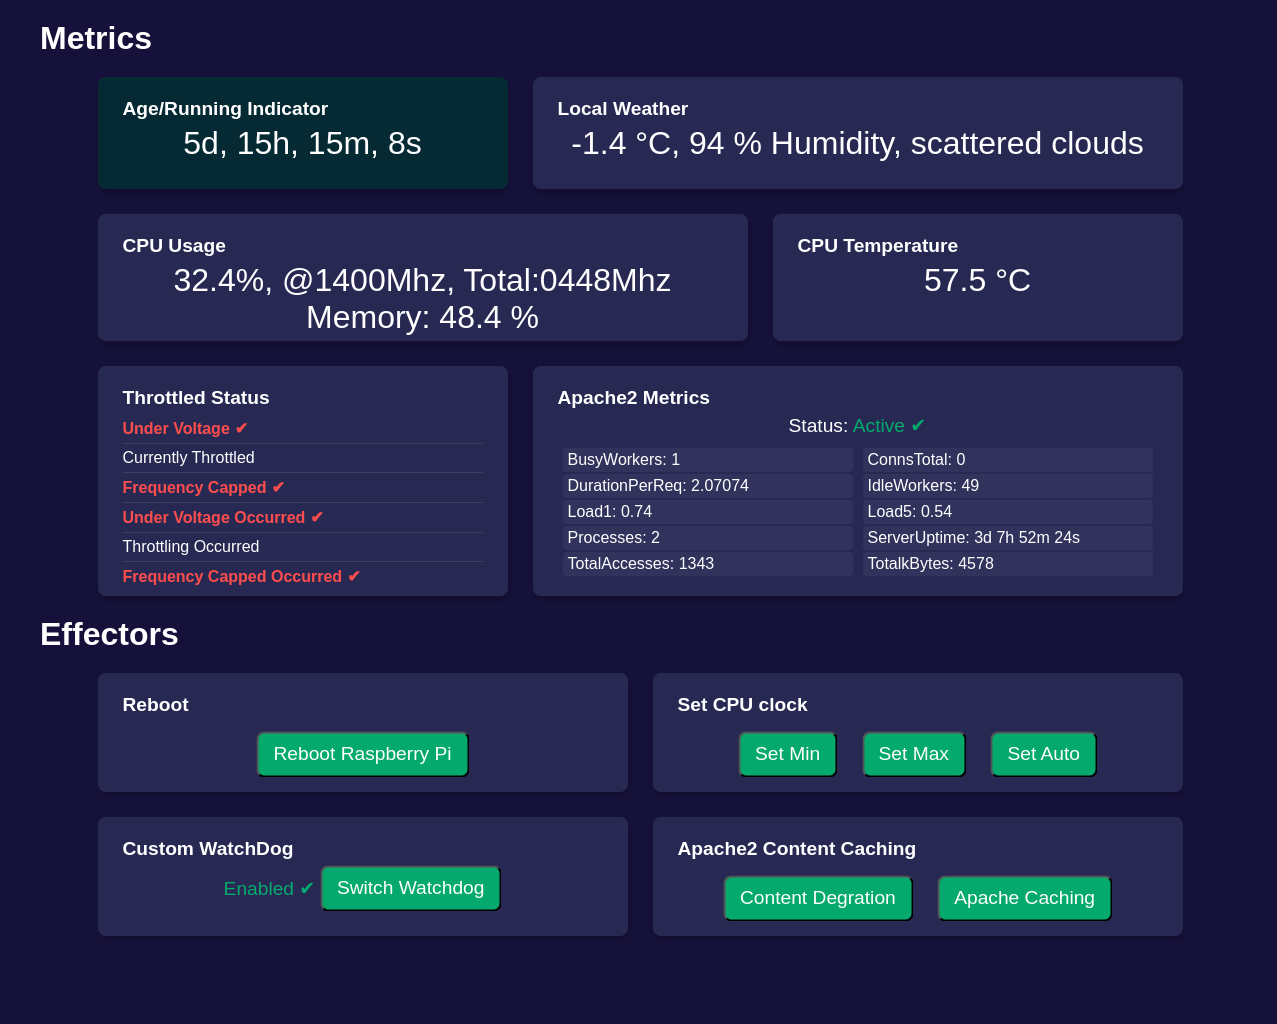
\includegraphics[width=0.45\textwidth]{./media/metrics_dashboard.png}
              \caption{Unbeatable Pi: Metrics and Effectors Dashboard}
              \label{fig:metrics_dashboard}
          \end{figure}

    \item \textbf{Analyze:}
          The analyze component is responsible for interpreting the metrics measured in the monitoring phase, in preparation for planning and the adaptation signal output. Two main approaches have been explored:

          \begin{itemize}
              \item \textbf{Utility Function:} The utility function asses two key areas. The first being machine health, focusing on CPU usage and temperature thresholds. The second, is website performance, focusing on network metrics. Table \ref{tab:utility-thresholds} summarizes the thresholds that were determined based on experimentation with the RPi. Initially, all metrics were to be considered, however, this approach was prone to bugs and thus, moving forward, only CPU Usage, Memory Usage, CPU Temperature, Apache Load, durationPerReq (Latency), and busyworkers are considered:
              
              \begin{table}[ht]
                \centering
                \caption{Adaptation Plans for System States}
                \label{tab:adaptation-plans}
                \small
                \begin{tabular}{cccc}
                \toprule
                \textbf{Plan No.} & \textbf{Serve Content} & \textbf{Serve Visitors} & \textbf{Downtime} \\
                \midrule
                1 & Full & All & No \\
                2 & Degraded & All & No \\
                3 & Degraded & Limited Number & No \\
                4 & X & X & rebooting \\
                \bottomrule
                \end{tabular}
                \end{table}

                To calculate utility, we assign weights to each metric based on their importance to achieving the adaptation goals. The utility component \( u_i \) for each metric is then calculated and a final utility score is found using Equation \ref{utility_formula},

                \begin{equation}
                U = w_{\text{CPU}} \cdot u_{\text{CPU}} + w_{\text{MEM}} \cdot u_{\text{MEM}}+ ...
                \label{utility_formula}
                \end{equation}

                where Equation \ref{utility_formula} is a shortened version of the full equation that would include all the relevant metrics.
                
              \item \textbf{Anomaly Detection:}
                    An Isolation Forest algorithm is trained on the historical data collected by the monitoring daemon. This algorithm isolates anomalies by looking at splits in data space that separate rare/unexpected points from normal ones. Over time, the aggregation of data should reveal a distinction between normal and unexpected operation. Using this model that is trained on this distinction, a check against the current data collected by the monitoring daemon is made. If the model identifies the data as an anomaly, then this serves as an indicator for the adaptation. To obtain this model, it was first necessary to prepare the data using the $prepare\_data.py$ script. Raw data from the monitoring daemon is preprocessed. Missing values are handled by dropping the rows. Categorical weather data was one-hot encoded to transform it into format that can be used for model training. Lastly, a StandardScaler is used to ensure uniformity in scale and improve model performance. Following the data preparation, the $train\_model.py$ script is invoked. This script takes the preprocessed data and uses it to train the Isolation Forest model that is used by the monitoring daemon for real-time detection. The contamination (expected portion of anomalies) hyperparameter was tweaked to 0.08, achieving a suitable balance for the model when working with our limited test data. The second hyperparameter, n\_estimators (number of trees), was left in its default value of 100.
          \end{itemize}
    \item \textbf{Plan:}
          The Utility function and Anomaly Detection both then select from set plans for adaptation. Plans, depend on which area has been identified as needing adaptation. There are four plans to consider. If machine health and website performance are both good, then CPU clock speeds are maximized for full content delivery. If the machine health is good, but website performance is bad, website content is degraded. Degradation methods include swapping dynamic content for static content, or lowering resolution on videos. If machine health is medium or critical, then the plan is to limit visitor connections or restrict content to text-only format. And lastly, if machine health is critical, the RPi is rebooted by the watchdog mechanism. These plans are illustrated by the state diagram of Figure \ref{fig:state_diagram}.

          \begin{figure}[H]
              \centering
              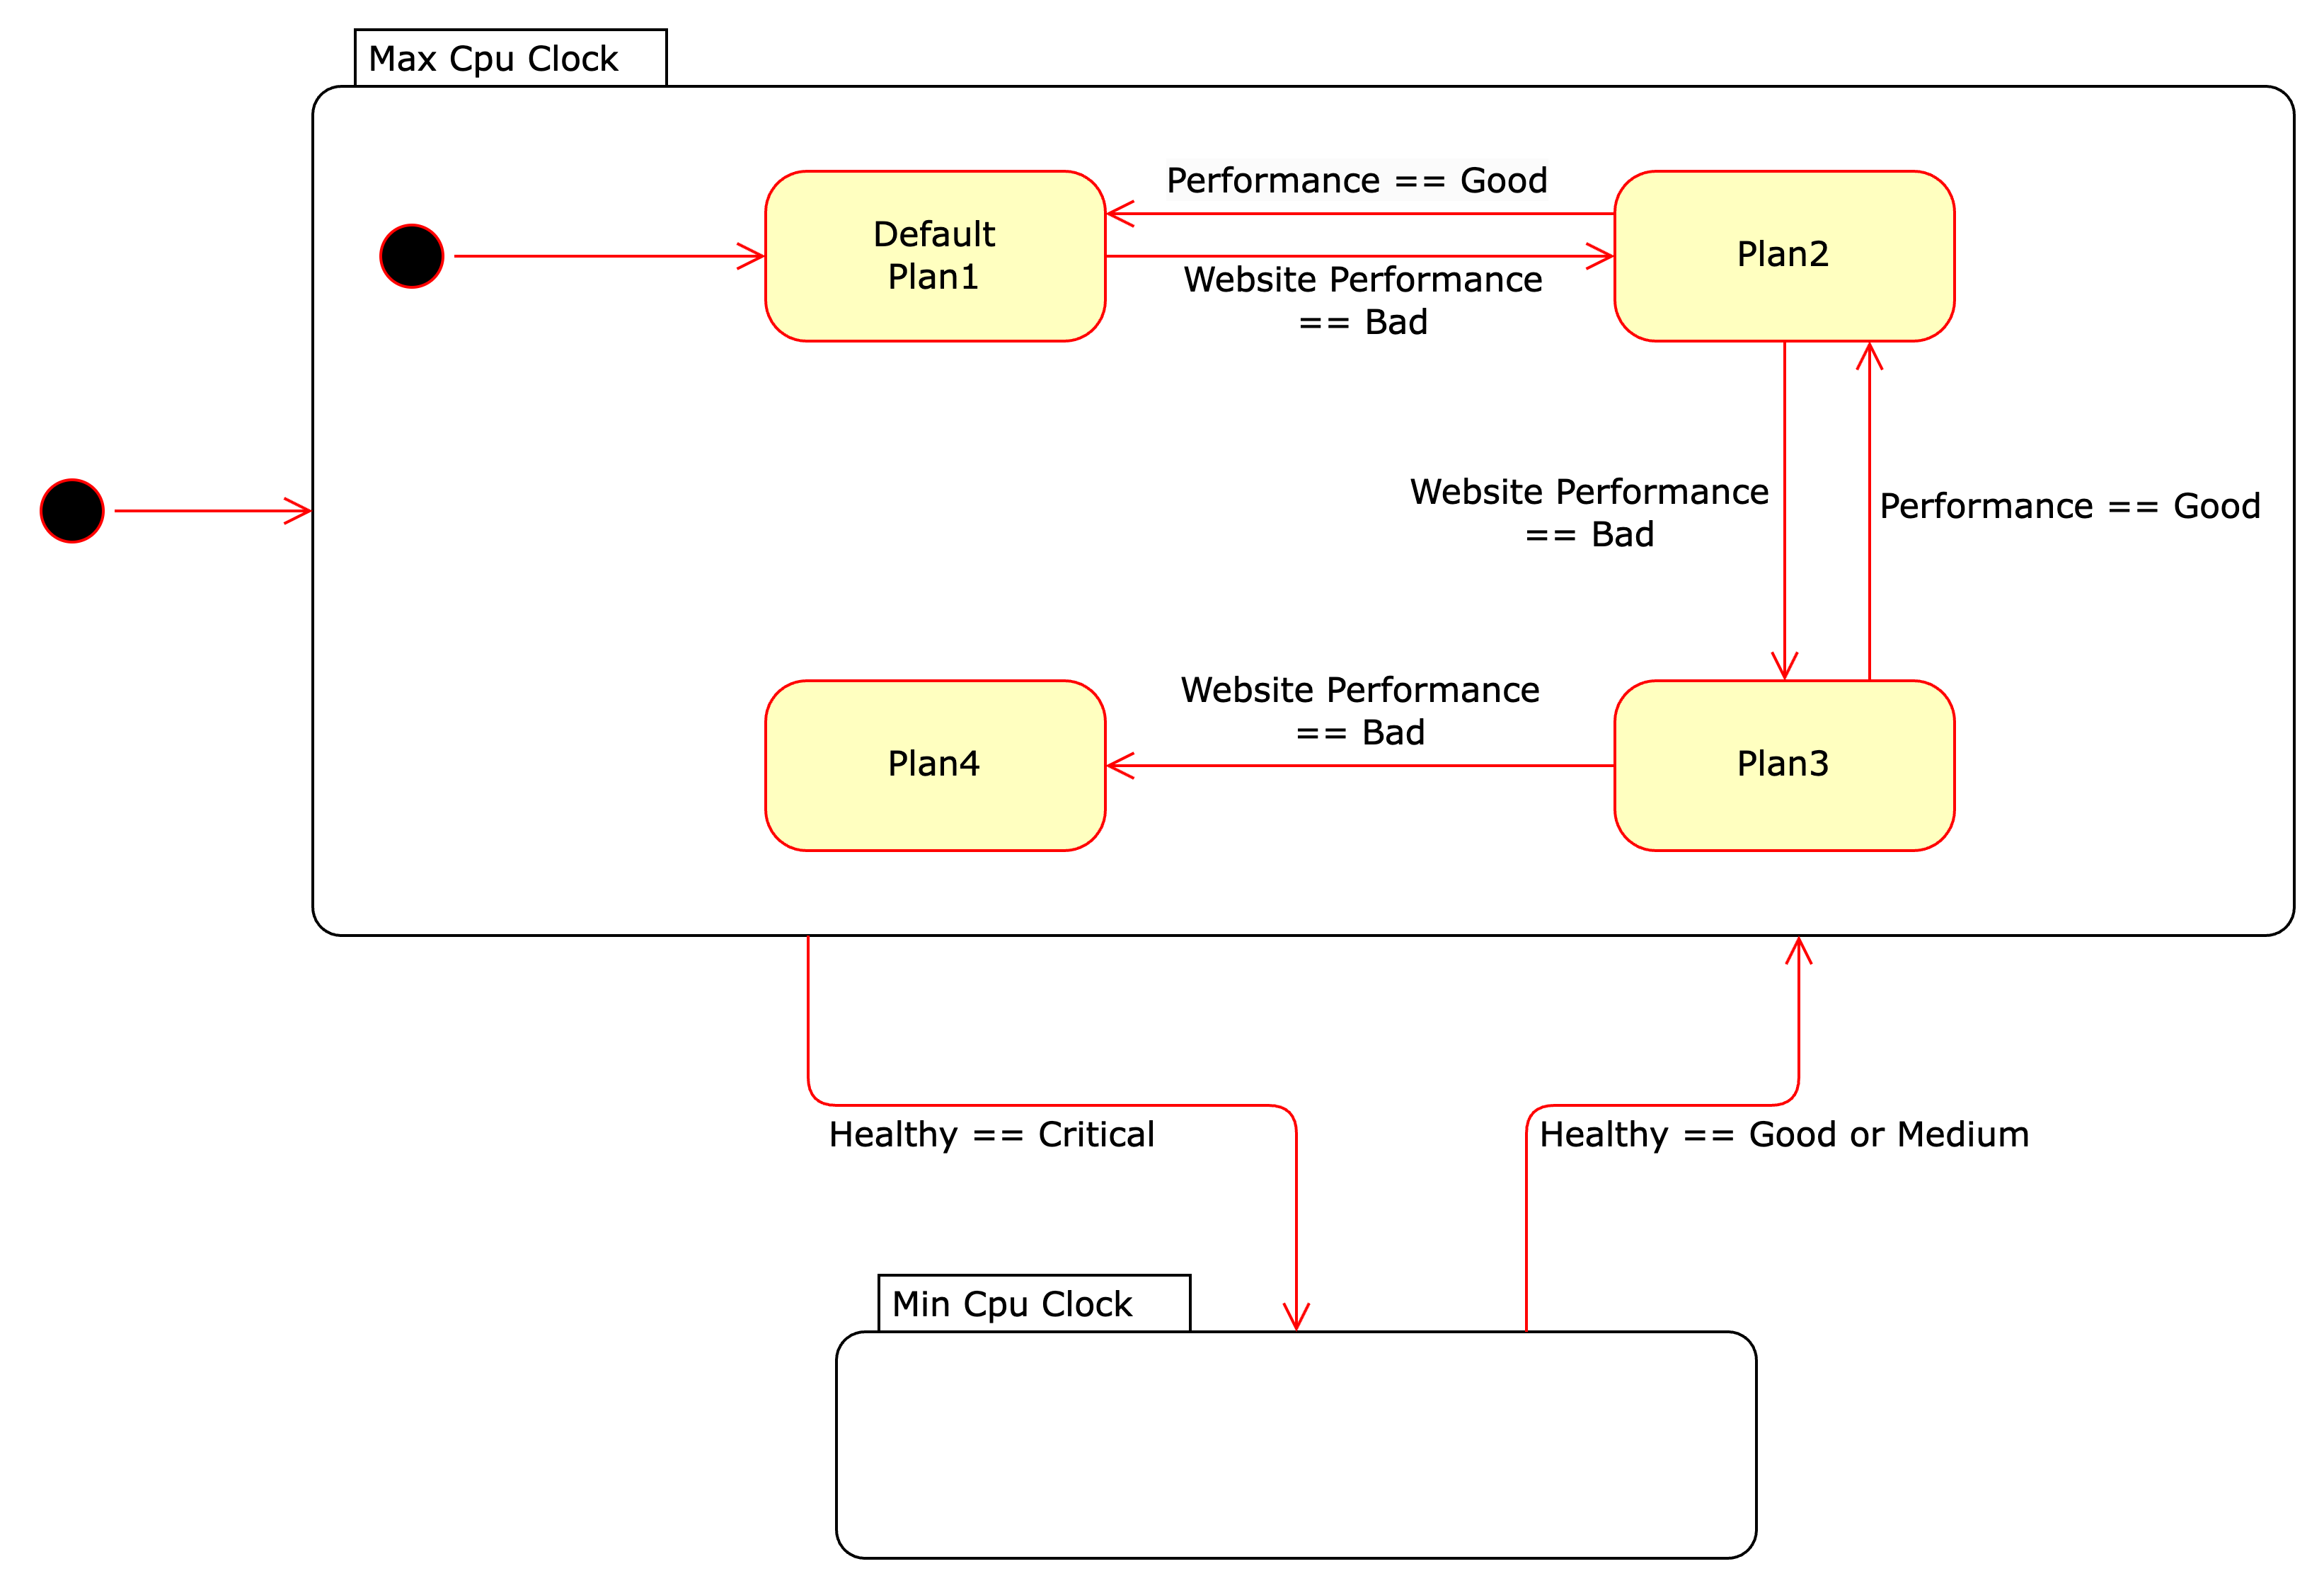
\includegraphics[width=0.45\textwidth]{./media/state_diagram.png}
              \caption{Unbeatable Pi: State diagram for adaptation plans}
              \label{fig:state_diagram}
          \end{figure}

    \item \textbf{Execute:}
          Using the same python libraries $psutil$ and $os$, it is possible to execute the plans to enact the system adaptation. For content degradation, a python script interacts with the HTML files served by Apache HTTP Server. By default, Apache2 does not have a direct APi interface to toggle the serving of media files, thus a script approach which modifies the .htaccess configuration file is taken, which does not require a restart or reload. Although the method results in some overhead to the server, its rare use makes the method still viable.
\end{itemize}

For added clarification, the environment, which is also monitored by the SAS, can be broken down into key components. The hardware constraints of the RPi itself and its specifications and external conditions are the two main environments that then encapsulate other components. The Apache HTTP Server which hosts the target website, connecting the RPi to users is an environment that connects the RPi to the external world/users.

Operation of the full feedback loop could be summarized as follows: the monitoring daemon starts by collecting system metrics and external metrics at a regular interval. These are the real-time snapshots of the system's state. The metrics collected are stored in a .csv file and evaluated against the thresholds defined by a utility function or alternatively, the Isolation Forest model. Each reading is evaluated and given a flag representing the health status (Good, Medium, or Critical) of both the machine and website performance. Based on the results, an appropriate adaptation plan is selected as described earlier. For example, the plan could be to increase CPU clock speed when both machine health and website performance are good. Lastly, the selected adaptation plan is implemented through the effectors.

This feedback loop implementation is illustrated by Figures \ref{fig:three_layer_framework} and \ref{fig:high_level_framework}. In Figure \ref{fig:three_layer_framework}, the adaptation goals are summarized in the Goal Management layer. Plans are then identified in the Change Management layer, and finally, the managed system and its various components are found in the Component Control layer. The Environment layer (not labelled) is found at the very bottom of the figure. In Figure \ref{fig:high_level_framework}, we are given another perspective of the framework and its various interactions between components in a more abstracted form.

\begin{figure}[H]
    \centering
    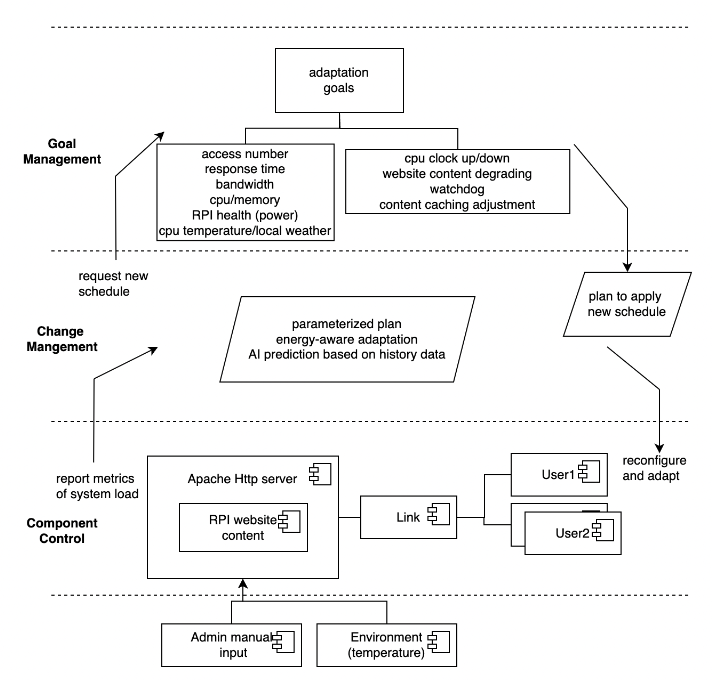
\includegraphics[width=0.45\textwidth]{./media/three_layer_framework.png}
    \caption{Unbeatable Pi: Three layer framework}
    \label{fig:three_layer_framework}
\end{figure}

\begin{figure}[H]
    \centering
    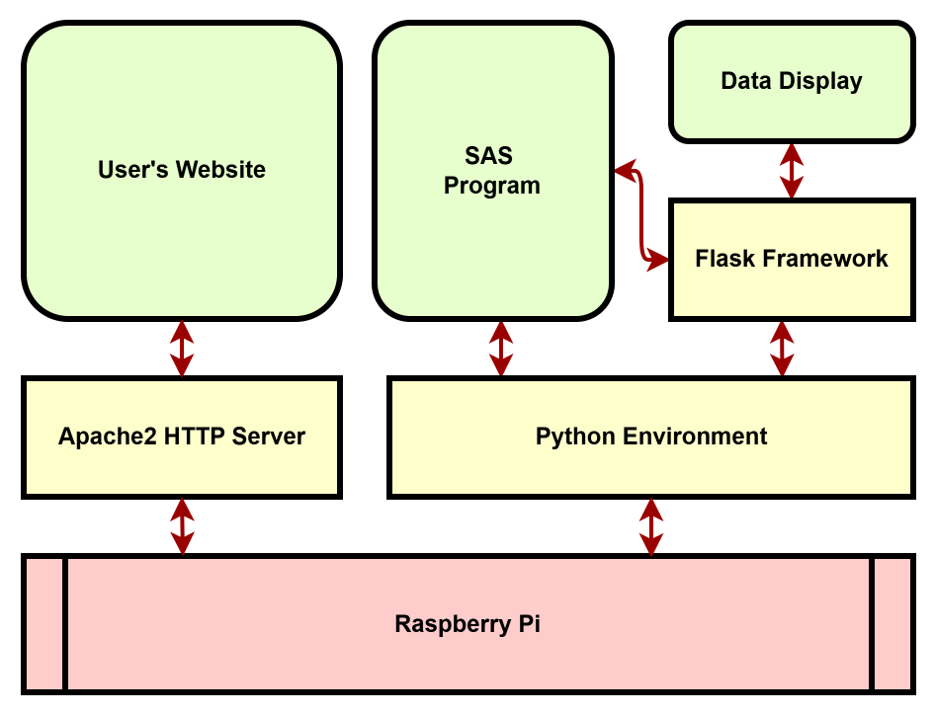
\includegraphics[width=0.45\textwidth]{./media/high_level_framework.png}
    \caption{Unbeatable Pi: High level conceptual framework}
    \label{fig:high_level_framework}
\end{figure}

For reference, the project's source code may be found in the GitHub repository \cite{arthur_github}. The many technologies mentioned (and others) are also briefly summarized by the following table:

\begin{table}[ht]
    \centering
    \caption{Summary of Technologies Used in the Project}
    \label{tab:technologies}
    \small
    \begin{tabular}{ll}
    \toprule
    \textbf{Technology} & \textbf{Purpose} \\
    \midrule
    RPi                    & Hardware platform hosting website \\
    Apache HTTP Server     & Hosts website and manages requests \\
    Python                 & Implementation language \\
    Flask                  & Framework for dashboard \\
    OpenWeather API        & Fetching environmental metrics \\
    psutil                 & Library for monitoring system metrics \\
    JMeter                 & Simulating web traffic and testing \\
    Isolation Forest       & ML algorithm for detecting anomalies \\
    StandardScaler         & Scaling data to improve model accuracy \\
    OneHotEncoder          & Encoding categorical data \\
    joblib                 & Serialization/deserialization of models \\
    \bottomrule
    \end{tabular}
    \end{table}
    
\section{\textbf{Testing and Results}}\label{test_and_results}
In order to test the adaptation system, a combination of Open-loop, JMeter and Stress-ng was used. Open-loop was used to perform a long running test to asses the system's base state and performance for comparison. We noted that the traffic and load on the RPi during idle operation is very light as depicted by Figure \ref{fig:idle_graphs}. CPU temps for example, remained low at 58 degrees Celsius, and CPU usage for example, remained stable at roughly 10\%, and no adaptation was triggered. JMeter, was used to simulate incoming traffic for various different loads. Two computers were running the JMeter scripts simultaneously in attempts to properly stress the RPiWeb. Two load types were used. The first setup is a ramp up to 600 threads (users), with an initial delay of 10 seconds to allow for additional configuration across computers. Initial users start at 5, with increments of 5 users every 1-2 seconds. The maximum load is then held for 180 seconds before the shutdown loop commences. The second script, has a sharper spike, shooting up to 500 threads and holding the load for a few minutes. Both scripts would at times run at the same time if the load on RPi was still minimal. Results of the test are depicted in Figure \ref{fig:heavy_load}. Specific implementations of the JMeter scripts ($traffic_simulation_spike.jmx$ and $traffic_simulation.jmx$) may be found in the GitHub repositories \cite{arthur_github}.

\begin{figure}[H]
    \centering
    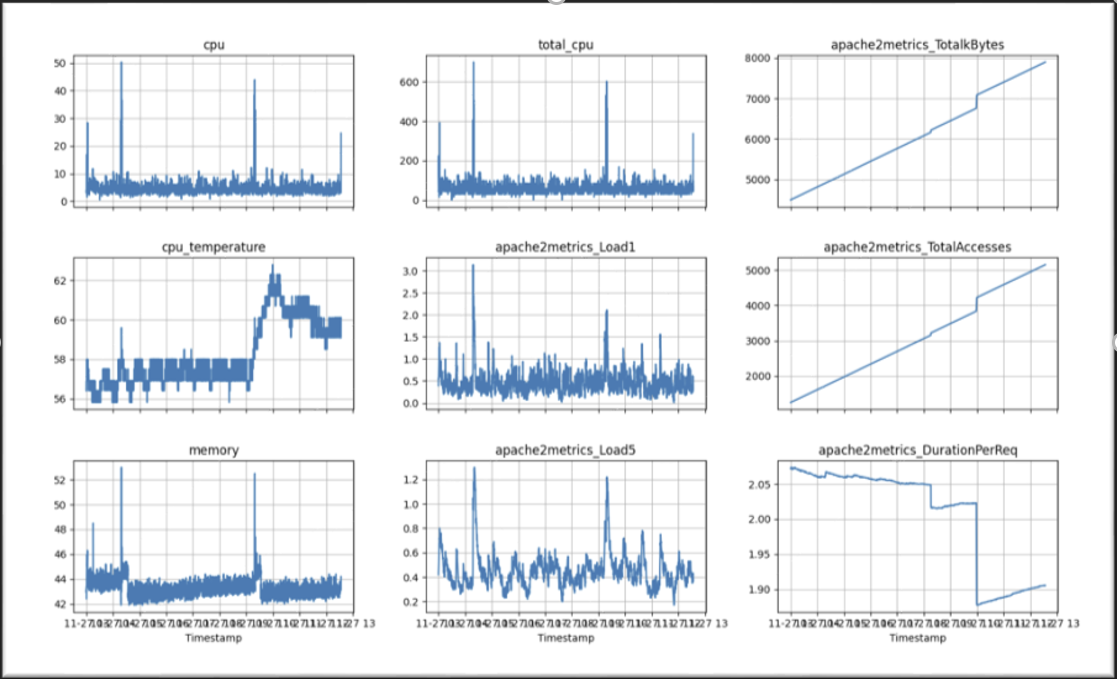
\includegraphics[width=0.45\textwidth]{./media/idle_graphs.png}
    \caption{Idle performance of RPi}
    \label{fig:idle_graphs}
\end{figure}

\begin{figure}[H]
    \centering
    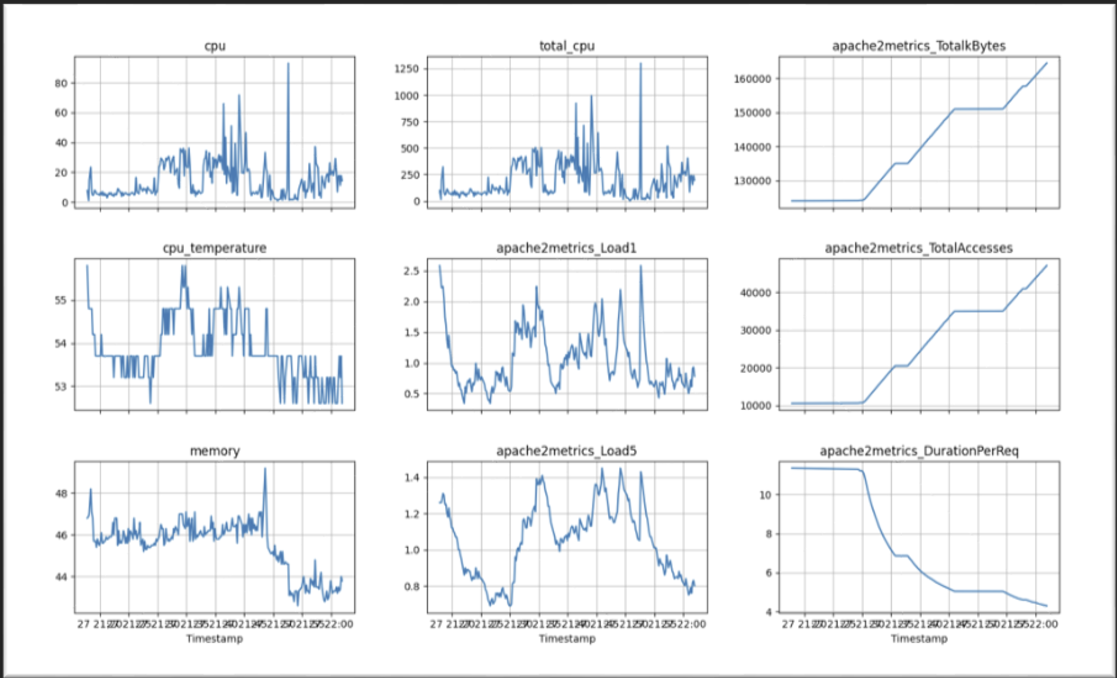
\includegraphics[width=0.45\textwidth]{./media/heavy_load.png}
    \caption{Heavy load on RPi}
    \label{fig:heavy_load}
\end{figure}

Finally, Stress-ng is used to take the RPi load to the extreme, representing the highest of load demand and triggering self adaptation. Figures \ref{fig:before_SAS_metrics} and \ref{fig:before_SAS_utility_and_plans} are from tests conducted with SAS disabled, while \ref{fig:after_SAS_metrics} and \ref{fig:after_SAS_utility_and_plans} are tests conducted with SAS enabled.

\begin{figure}[H]
    \centering
    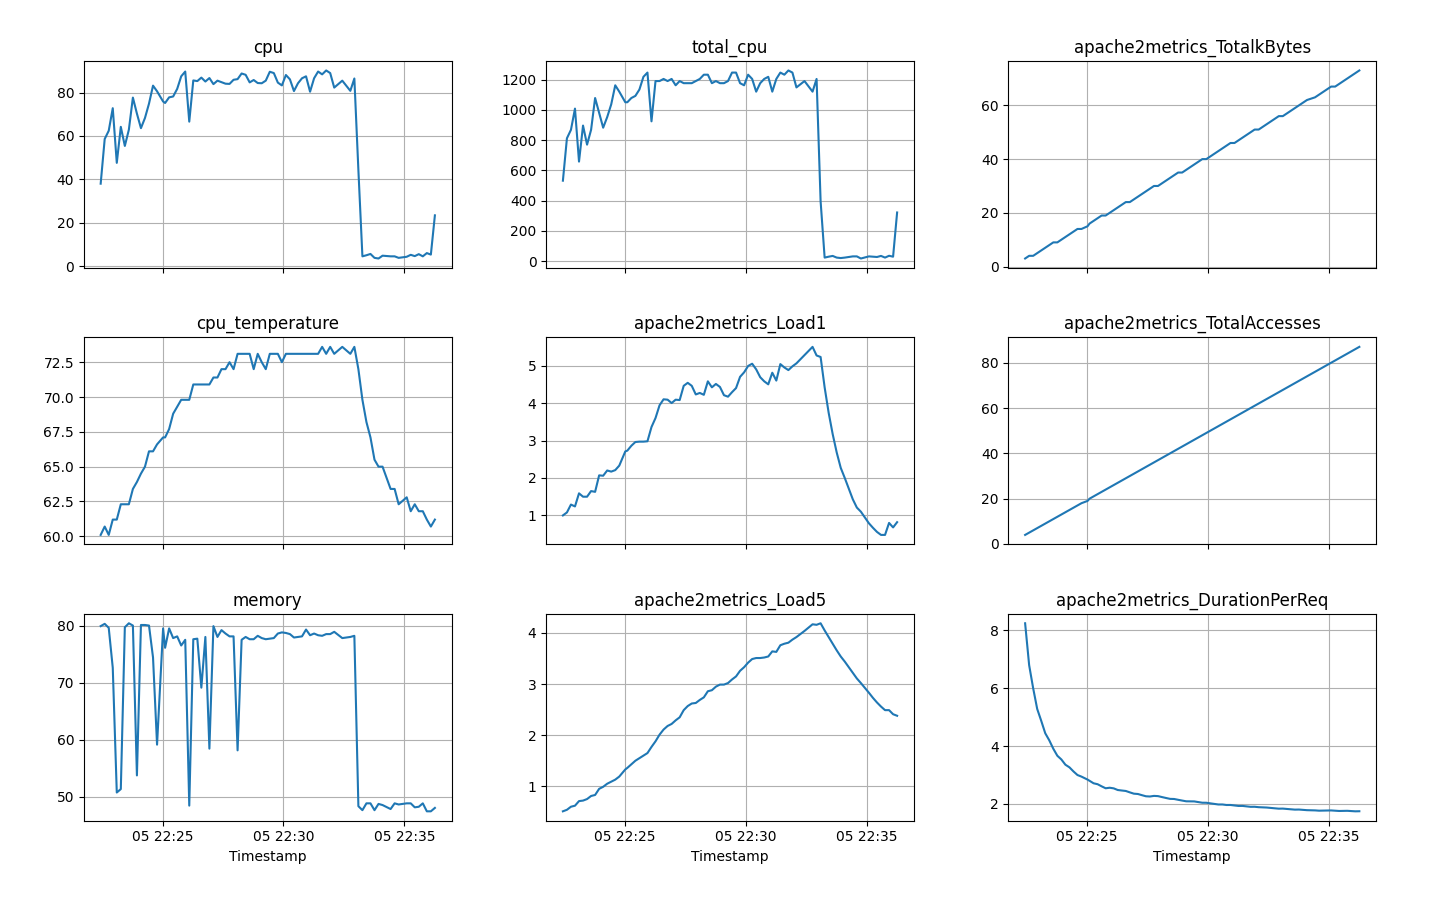
\includegraphics[width=0.45\textwidth]{./media/before_SAS_metrics.png}
    \caption{RPi system metrics with SAS disabled}
    \label{fig:before_SAS_metrics}
\end{figure}

\begin{figure}[H]
    \centering
    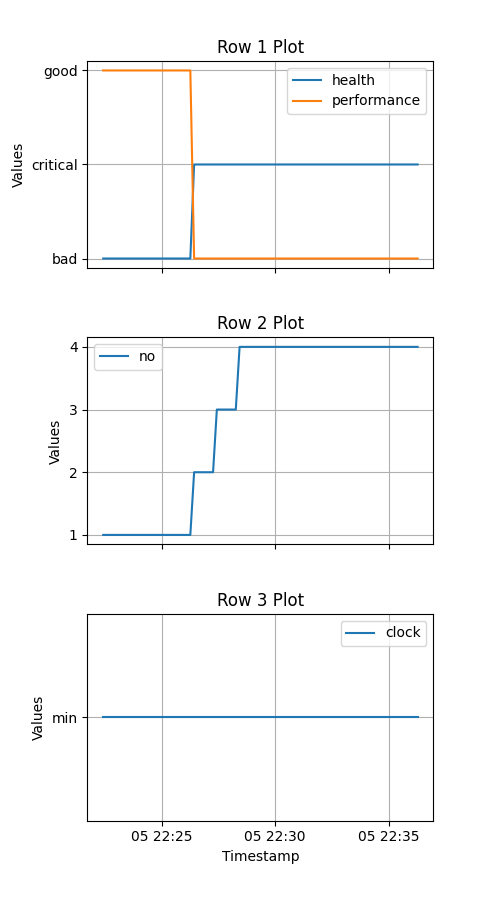
\includegraphics[width=0.45\textwidth]{./media/before_SAS_utility_and_plans.png}
    \caption{Utility and adaptation plans with SAS disabled}
    \label{fig:before_SAS_utility_and_plans}
\end{figure}

With SAS disabled, all metrics are high; cpu usage remains at values above 80\%, with CPU temperatures reaching 72 degrees Celsius. Memory usage hits values of 80\% and is very unstable. In terms of the system utility and adaptation plans, Figure \ref{fig:before_SAS_utility_and_plans} shows that system health remains critical throughout the test and website performance is also bad throughout.

\begin{figure}[H]
    \centering
    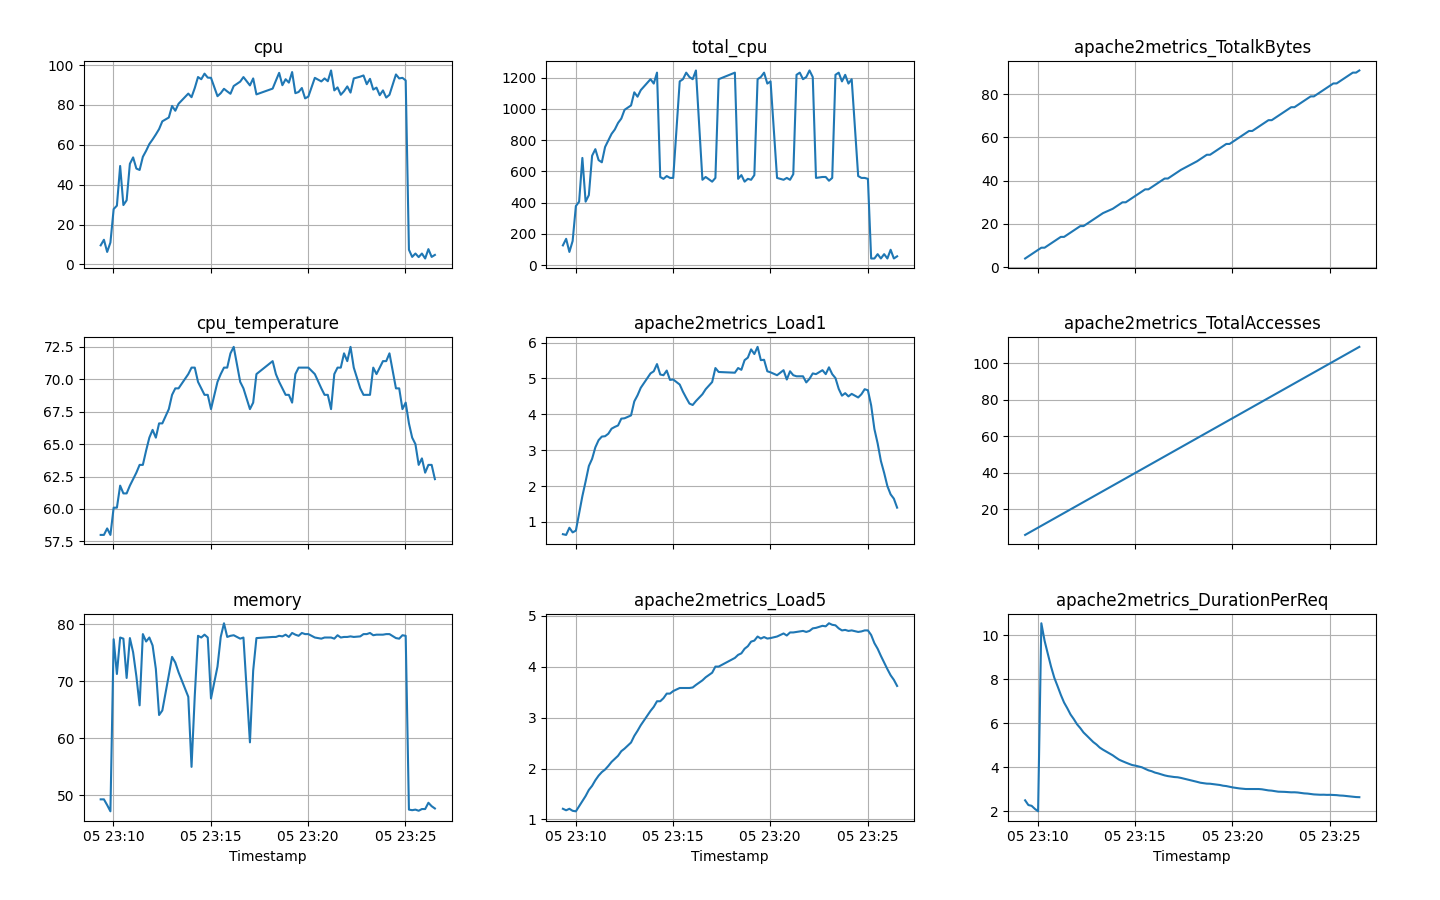
\includegraphics[width=0.45\textwidth]{./media/after_SAS_metrics.png}
    \caption{RPi system metrics with SAS enabled}
    \label{fig:after_SAS_metrics}
\end{figure}

\begin{figure}[H]
    \centering
    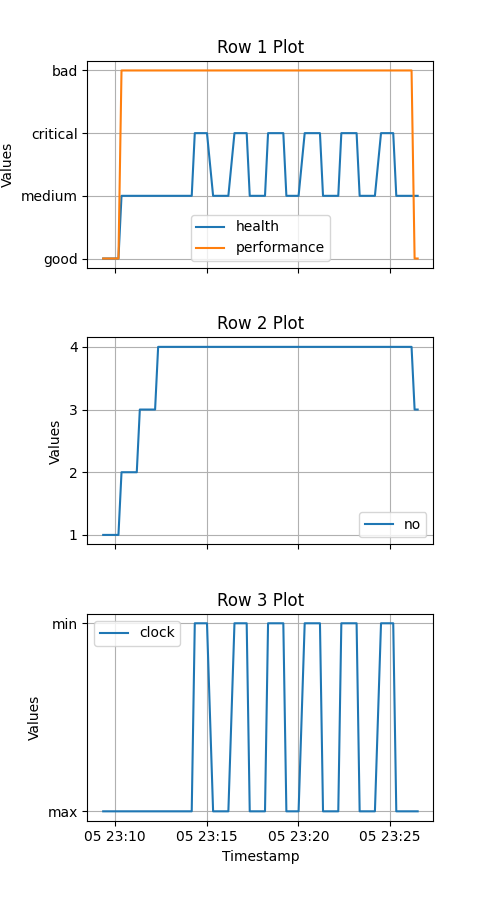
\includegraphics[width=0.45\textwidth]{./media/after_SAS_utility_and_plans.png}
    \caption{Utility and adaptation plans with SAS enabled}
    \label{fig:after_SAS_utility_and_plans}
\end{figure}

With the SAS system enabled, CPU usage did not see major improvements, however total CPU saw some improvements. CPU temperature experiences the best improvement under SAS. Previously, temperatures would continue to rise due to the continued high load on the system. However, with SAS enabled, this constant load is reduced, allowing the system to breathe and somewhat reducing temperatures overall. Latency before and after remained relatively the same, which is indicative of the overhead of SAS does not heavily affect the website performance when activated. In terms of the utility, the system no longer remained in a prolonged critical state for system health, with network performance unchanged.



\begin{thebibliography}{00}

    \bibitem{pi_sales} L. Pounder, "Raspberry Pi celebrates 12 years as sales break 61 million units," Tom's Hardware, Feb. 29, 2024. [Online]. Available: \url{https://www.tomshardware.com/raspberry-pi/raspberry-pi-celebrates-12-years-as-sales-break-61-million-units}. [Accessed: Dec. 4, 2024].

    \bibitem{magic_mirror} L. Upton, "Magic Mirror," Raspberry Pi Foundation, Apr. 29, 2014. [Online]. Available: \url{https://www.raspberrypi.com/news/magic-mirror/}. [Accessed: Dec. 4, 2024].

    \bibitem{pi_history} "Industrial Raspberry Pi: A brief history and current state," OnLogic, Mar. 14, 2024. [Online]. Available: \url{https://www.onlogic.com/blog/industrial-raspberry-pi-a-brief-history-and-current-state/}. [Accessed: Dec. 4, 2024].

    \bibitem{pi_headaches} https://www.makeuseof.com/raspberry-pi-difficulties-self-hosting-services/

    \bibitem{pi_website_hosting} https://fastercapital.com/content/Web-Server--Hosting-a-Website-with-Raspberry-Pi.html\#Troubleshooting-common-issues-when-hosting-a-website-with-Raspberry-Pi

    \bibitem{pi_vs_AWS} https://nelop.com/comparing-a-raspberry-pi-4-to-aws/

    \bibitem{IBM_mainframes} https://www.datacenterdynamics.com/en/news/ibm-mainframes-survive-48-magnitude-earthquake-in-us-east-coast/

    \bibitem{arthur_github} https://github.com/ArthurQiangLi/Lets\_SAS\_RPI\_Websites/tree/main


\end{thebibliography}

\end{document}
